\chapter[Numerical Integration of the Maxwell-Bloch Equations]
  {Numerical Integration of the\\ Maxwell-Bloch Equations}
  \label{apx:mb_eqns}

  % \section{Intro}

    In this appendix we describe the design and implementation of numerical
    methods to solve the coupled Maxwell-Bloch (\textsc{mb}) equations
    describing the nonlinear propagation of near-resonant light through thermal
    atomic vapours. The derivation of the \textsc{mb} equations is given in
    chapter \ref{chp:propagation} and simulated results from the scheme here
    described are presented throughout the thesis.

  \section{Formulating the Problem}

    The \textsc{mb} equations are together equations (\ref{eqn:comoving_mwe})
    and (\ref{eqn:lindblad}), which we will restate here for completeness. They
    are the first-order Maxwell wave equation with the slowly-varying envelope
    approximation
    \begin{equation*}
      \frac{\partial}{\partial z} \mathcal{E}(z,t') = 
        \mathrm{i} \frac{k}{2 \epsilon_0}
        N(z) \sum_{i \ne j} d_{ij} \int_{-\infty}^{\infty} 
          \rho_{ij}(z,t; v) f(v) {\dd v}. 
    \end{equation*}
    describing propagation of the field envelope and the Lindblad master
    equation
    \begin{equation*}
      \ii \hbar \frac{\partial \rho}{\partial t} = [\mathcal{H}, \rho] + 
        \mathcal{L}\left\{ \rho \right\}
    \end{equation*}
    describing the time-evolution of the atomic density matrix interacting with
    that field.

    We describe the problem in the natural unit system defined in section
    \ref{sec:propagation_two}, in terms of the length of the medium $L$, the
    natural linewidth of the transition $\Gamma$ (specifically the probe
    transition in the case of schemes with multiple field modes) and its
    reciprocal natural decay time $\tau = \nicefrac{1}{\Gamma}$. Our goal is to
    solve the \textsc{mb} equations over a domain in \textsc{1d} space $z \in
    [0, 1]$ and co-moving time $t' \in [t_{\mathrm{min}}, t_{\mathrm{max}}]$.

    We begin by setting up a discrete lattice over $z$ and $t'$, with $N_z$
    equal spacesteps of length $h_z = 1/N_z$, such that $z_j =  j \cdot h_z ~
    \forall j \in \{0, 1, 2, \dots, N_z\}$ and $N_t$ equal timesteps of duration
    $h_t = 1/N_t$, such that $t_k =  k \cdot h_t ~ \forall k \in \{0, 1, 2,
    \dots, N_t\}$.

    The overall strategy is then to calculate values for the discretised
    electric field $\mathcal{E}_{j,k}$ across the lattice, for which we must
    determine the macroscopic polarisation $\mathcal{P}_{j,k}$ of the atoms,
    which in turn is derived from the density matrix $\rho_{j,k}$.  A self-
    consistent algorithm is required for computation. Note that the electric
    field and polarisation envelopes in general consist of multiple modes,
    representing polarisations and wavelengths resonant with different
    transitions. For clarity in describing the scheme we will present only a
    single mode $\mathcal{E}_{j,k}$, but describe how the algorithm is extended
    to multiple modes later on.

    We define a discrete set of detunings $\{\Delta_l\}$, representing atoms
    across a range of Doppler-shifted velocity classes. This range should be
    broad enough to cover the Maxwell-Boltzmann probability distribution and
    dense enough to accurately map the spectral absorption window. We will
    discuss those accuracy requirements in section \ref{sec:mb_accuracy}.

    Any formulation of an integration scheme for partial differential equations
    is complete only with the definition of appropriate boundary conditions.
    Here we take a boundary condition for the field at the front of the medium
    (\ie $j\!=\!0$) defining the field profile over time input on the medium
    $\mathcal{E}_{j=0, k}$. In a typical simulation of experiment this might be
    a pulse or a ramp-on to a \textsc{cw} field. We must also specify an initial
    condition for the density matrix $\rho_{j, k=0}$. Typically we set this such
    that all population starts off in the atomic ground state.

  \section{Computational Scheme}

    \begin{figure}
      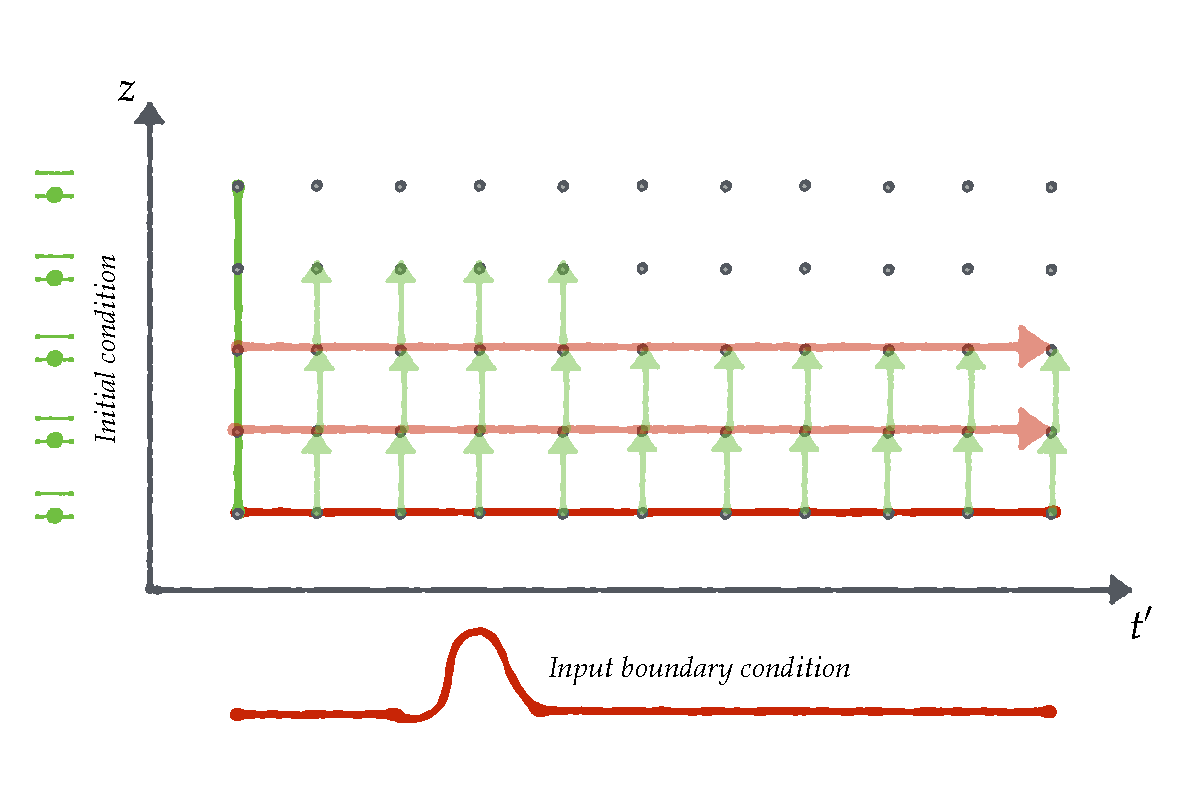
\includegraphics[width=\linewidth]{figs/10_appendices/mb_scheme.pdf}
      \caption{
      Finite difference integration scheme for the Maxwell-Bloch equations. The
      equations are solved for a discrete lattice over space $z$ and co-moving
      time $t'$. At each lattice point ($z_j,t_k'$) we wish to solve for the
      electric field $\mathcal{E}(z_j,t_k')$ and the atomic density matrix
      $\rho(z_j,t_k')$. The initial condition is illustrated by the two- level
      icons on the left. The boundary condition defining the electric field
      pulse profile over time input on the medium is illustrated by the sketched
      pulse at the bottom.
      }
      \label{fig:mb_scheme}
    \end{figure}

    \begin{algorithm}
    \caption{Maxwell-Bloch integration.}
    \label{alg:mb}
    \begin{algorithmic}[1]
        \For{$j = 2$ to $N_z$} \Comment{Loop over spacesteps}
            \For {$l = 0$ to $N_\Delta$} \Comment{Loop over velocity classes}
              \State $\rho^l_{j} = \mathrm{solve\_lindblad}(\rho_\mathrm{init}, 
                \mathcal{E}_j, \Delta_l)$
            \EndFor
            \For{$k = 0$ to $N_t$} \Comment{Loop over timesteps}
              \State $\mathcal{P}_{j,k} = 
                \mathcal{N}_z \sum_{a \ne b}\int_{l} d_{ab} 
                \rho^l_{j,k} [a,b] f(\Delta_l, u) \dd \Delta$
              \State $\mathcal{E}_{j+1,k} = 
                \mathcal{E}_{j+1,k} + \ii h_z \frac{k}{2 \varepsilon_0}
                \left[ \frac{3}{2} \mathcal{P}_{j,k} - \frac{1}{2} 
                \mathcal{P}_{j-1,k} \right]$
              \Comment{The \textsc{ab} step}
            \EndFor
        \EndFor
    \end{algorithmic}
    \end{algorithm}

    The finite difference scheme is illustrated in figure \ref{fig:mb_scheme}
    and sketched out with pseudocode in algorithm \ref{alg:mb}. For each
    spacestep index $j$ in the medium, we take the field $\mathcal{E}_{j,k}$
    arriving on that step for all timesteps $t'_k$. For the first spacestep
    ($j\!=\!0$) this is the input boundary condition, illustrated in red in
    figure \ref{fig:mb_scheme}. Next (lines 2--4 in the pseudocode) we loop over
    the velocity classes $l$ and pass the detuning $\Delta_l$, the field profile
    $\mathcal{E}_{j,k}$ and an initial condition ($\rho_\mathrm{init}$) to an
    \textsc{ode} solver for the Lindblad master equation. That solver contains
    an implicit loop through the $N_t$ timesteps, and integrates the Lindblad
    equation to find the density matrix at each of those timesteps $t'_k$.

    At this point we have solved for the density matrix $\rho^l_j$ at the
    spacestep $z_j$ for each time $t_k$ and for atoms in each velocity class
    $l$. In a loop over the timestep index $k$ (lines 5--8) we then perform an
    average of the density matrix coherences over detuning, weighted by the
    Maxwell-Boltzmann probability distribution for a defined width $u$, and sum
    them to find (line 6) the polarisation $\mathcal{P}_{j,k}$ at that point in
    space $z_j$ and time $t_k$.

    Once we have computed the polarisation, and still within the loop over
    timesteps, we can advance the field at that timestep to the next spacestep
    $\mathcal{E}_{j+1,k}$ in the medium for each $k$ using a second-order
    Adams-Bashforth method. Note then that this method is not strictly
    chronological, but is self-consistent in the co-moving frame of reference.

    \subsection{Details of the Algorithm}

    The pseudocode above describes the general calculation scheme, but omits a
    number of details that we will now describe.

    First, we have considered only a single field mode. For multiple modes, we
    must input all of those modes to the Lindblad solver (in line 3). We must
    also calculate polarisations for each mode separately from its coupled
    transitions (line 6) and advance the fields for each mode (line 7).

    Second, note that we started the spacestep loop (line 1) at $j\!=\!2$. The
    two-step Adams-Bashforth method requires two starting points to begin. We
    therefore use an explicit Euler step to take the input field at $j\!=\!0$ to
    the next step at $j\!=\!1$. As the local error in the Euler step is of order
    $\mathcal{O}(h_z)$, we use a smaller step to avoid introducing a large
    global error. The second step is then a two-step Adams-Bashforth with
    different stepsizes. The correct difference formula for this step
    (\ref{eqn:ab_step_different}) is derived in Appendix \ref{apx:ab_method}.
    The remaining steps use the standard two-step Adams-Bashforth step as shown
    in the pseudocode.

    Third, the Lindblad solver (line 3) requires the electric field envelope
    $\mathcal{E}_j$ to be passed as a function of time, rather than an array, as
    the adaptive method may choose different inner stepsizes (\ie steps between
    $t'_k$ and $t'_{k+1}$ for any $k$) that we do not know in advance. We
    construct this function for arbitary points in the time domain using
    quadratic spline interpolation.\cite{press2007numerical,DeBoor1972}.

    Fourth, the complex values for the field envelopes $\mathcal{E}_{j,k}$ and
    atomic density matrix $\rho_{j,k}$ across the lattice is saved to disc in
    binary format, such that the results of each simulation can be loaded
    without needing the calculation to be repeated. To optimise storage and
    memory requirements, a data resolution in $z_h$ and $t_k$ may be specified,
    sufficient for analysis and visualisation without needing to record all of
    the steps that may be required for stability and accuracy.

    Spectral analysis of the results is performed using a discrete Fourier
    transform of the complex field.\cite{press2007numerical}   

    \subsection{Code Implementation}

    The algorithm for solving the \textsc{mb} equations was implemented in
    Python using the \textit{SciPy} scientific computing
    stack\cite{VanDerWalt2011,Jones}.

    The code uses the \texttt{OB} class of the \textit{OpticalBloch} package in
    order to define the atom-light interaction and solve the Lindblad equation
    for instances representing various atomic systems, with few-level or with
    full angular momentum structure. The \textit{QuTiP} library\cite{Nation2013}
    is used for quantum state and operator objects and its master equation
    solver for dynamics of open quantum systems.

  \section{Convergence \& Accuracy}\label{sec:mb_accuracy}

    We check the accuracy of the method with a quantitative measurement of the
    convergence of results for a particular system with increased number of
    spacesteps and velocity classes. We wish the results to be as accurate as
    possible, but with an awareness of the trade-off that the computational
    complexity (and thus running time) scales with $\mathcal{O}(N_z)$ and
    $\mathcal{O}(N_\Delta)$ where $N_\Delta$ is the number of velocity classes.

    \begin{figure}
      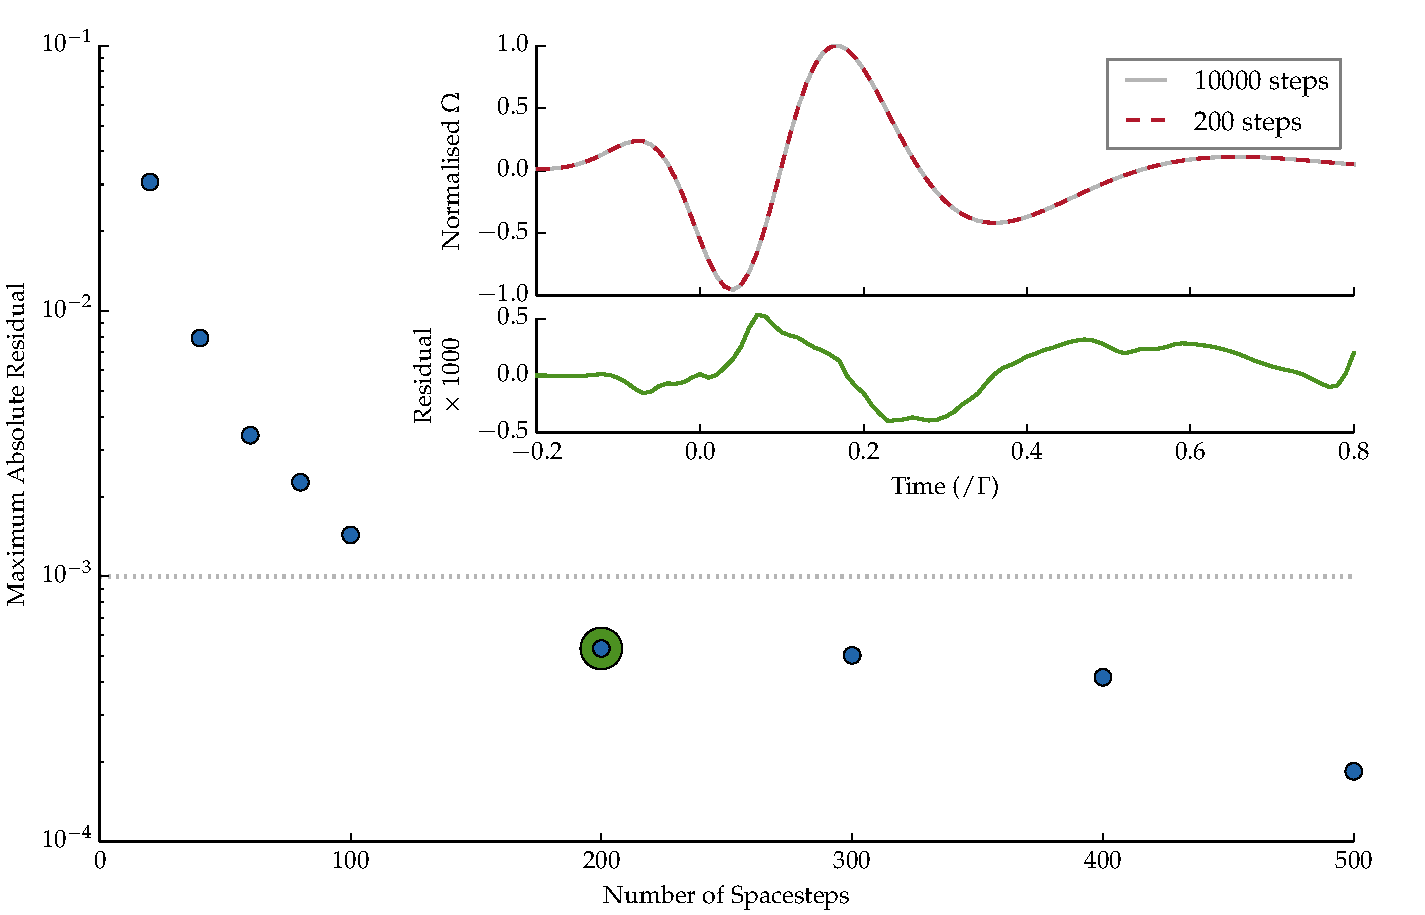
\includegraphics[width=\linewidth]{figs/10_appendices/two_mb_solve_h_compare_fig1.pdf}
      \caption{
      Convergence of an example integrated solution, for a weak pulse in a
      medium with $\mathcal{N}g = \unit[2\pi~100]{MHz}$, for different numbers
      of spacesteps $N_z$. (Main plot) The minimum absolute residual between an
      integrated solution $N_z$ and a benchmark solution with $10,000$ steps
      (blue circles), plotted on a logarithmic $y$-axiz. The dotted line
      represents a chosen accuracy requirement of $10^{-3}$ and the green
      circled data point is the lowest number of steps tested which meets this
      requirement, in this case $N_z = 200$. (Inset) Normalised $\Omega$ against
      time at the final spacestep $j = N_j$ for both the benchmark and the $N_z
      = 200$ run, with the residual shown underneath.
      }
      \label{fig:steps_convergence}
    \end{figure}    

    In figure \ref{fig:steps_convergence} we show the results of convergence of
    the integrated solutions for different numbers of spacesteps $N_z$ between
    $10$ and $500$. The convergence is measured relative to a benchmark at
    $10,000$ spacesteps --- a number which ensures high accuracy but is too slow
    for performing many calculations. The maximum value of the absolute
    difference (residual) between the benchmark and each run is plotted. We see
    that the maximum absolute residual decreases with the number of steps $N_z$
    down to $200$ steps, after which the increase in accuracy for an
    increased number of steps is reduced. If we choose a tolerance for the
    maximum absolute residual of $10^{-3}$ (shown by the dotted line), the first
    tested run within that tolerance is $N_z = 200$. Running simulations with
    this number of spacesteps would therefore reduce calculation many times over
    the benchmark while keeping a sufficient level of accuracy.

    \begin{figure}
      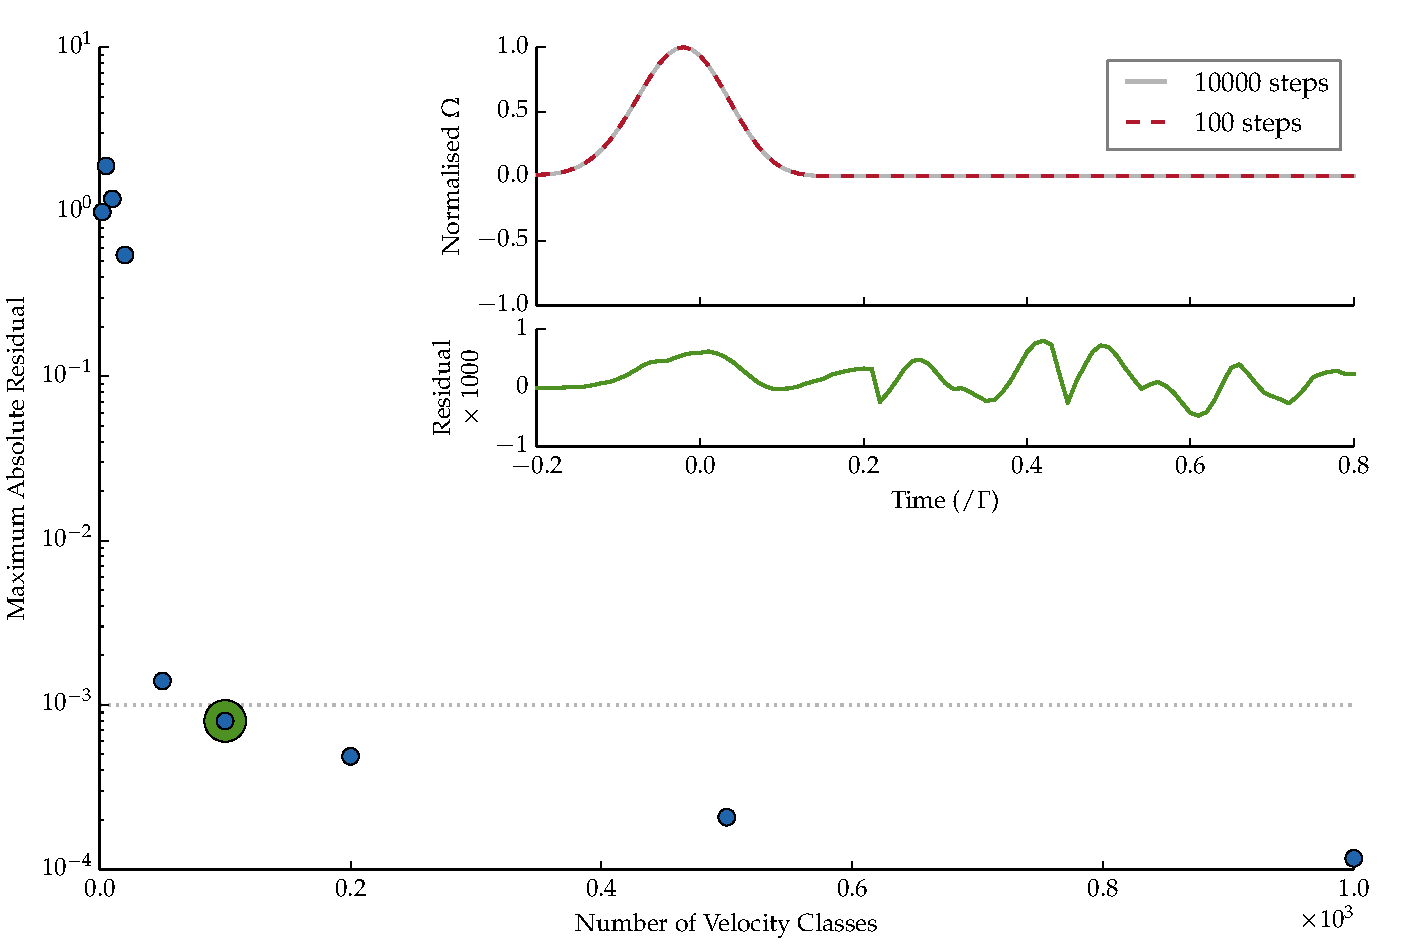
\includegraphics[width=\linewidth]{figs/10_appendices/two_mb_thermal_solve_j_compare_fig1.pdf}
      \caption{
      Convergence of an example integrated solution, for a weak pulse in a
      medium with $\mathcal{N}g = \unit[2\pi~100]{\Gamma/L}$ and a thermal width
      of $\unit[2\pi~10]{\Gamma}$, for different numbers of velocity classes
      $N_\Delta$. (Main plot) The minimum absolute residual between an
      integrated solution $N_\Delta$ and a benchmark solution with $10,000$
      velocity classes, plotted on a logarithmic $y$-axis. The dotted line
      represents a chosen accuracy requirement of $10^{-3}$ and the green
      circled data point is the lowest number of steps tested which meets this
      requirement, in this case $N_\Delta = 100$. (Inset) Normalised $\Omega$
      against time at the final spacestep $j = N_j$ for both the benchmark and
      the $N_\Delta = 100$ run, with the residual shown underneath.
      }
      \label{fig:vel_convergence}
    \end{figure}

    In figure \ref{fig:vel_convergence} we show a similar figure for results of
    convergence for the integrated solutions for different numbers of velocity
    classes $N_\Delta$ between $1$ and $1,000$ spread over a width of
    $\unit[2\pi~40]{\Gamma}$.

    The convergence is measured relative to a benchmark at $10,000$ velocity
    classes.  We see that the maximum absolute residual is large for few
    velocity classes, around $1$. If we again choose a tolerance for the maximum
    absolute residual of $10^{-3}$ (shown by the dotted line), the first tested
    run within that tolerance is $N_z = 100$. The `return on investment' for
    additional velocity classes is reduced from then on, with $N_z = 1,000$ not
    providing an order of magnitude improvement in accuracy.

    In picking a range of velocity classes for an accurate simulation, there are
    two important considerations. First, it is important to cover the Maxwell-
    Boltzmann distribution. We check the integration width is sufficient by
    using a simple trapezoidal integration over the discrete Maxwell-Boltzmann
    distribution to ensure it is close to unity. In each of the calculations
    above we used an evenly-spaced sampling over four times the \textsc{fwhm}.
    The integral is far from unity until around $20$ detuning steps (when it
    reaches $0.995$), which explains why we don't see convergence in the first
    few samples.  Second, it is important to sample accurately the Lorentzian
    resonance window, which is typically much smaller than the thermal width (in
    our case it is specified to be $\unit[2\pi~1]{\Gamma}$). In order to achieve
    both of these goals with an optimised number of detuning steps, we use a
    non-evenly spaced grid with a denser number of velocity classes around
    resonance, which can improve accuracy without requiring as many velocity
    classes.

  \section{Parallelisation \&  Performance}

    The pseudocode in algorithm \ref{alg:mb} contains a number of nested loops,
    which leads us to consider if any parts of the implementation may readily be
    parallelised. 

    The iterations of the outermost loop over spacesteps $z_j$ (algorithm
    \ref{alg:mb}, line 1) are not independent (\ie the field at a point in space
    $j$ is dependent on the previous space points $0, 1, \dots, j-1$) which
    necessitates that these be processed in serial. However, the iterations of
    the inner loop over velocity classes $\Delta_l$ (algorithm \ref{alg:mb},
    line 2), calculate the evolution of atoms subject to different Doppler
    shifts with respect to the fields along $z$. The evolution of each class is
    completely independent of the others so these may be processed in parallel,
    with the weighted average calculated at the end.

    \begin{figure}[]
      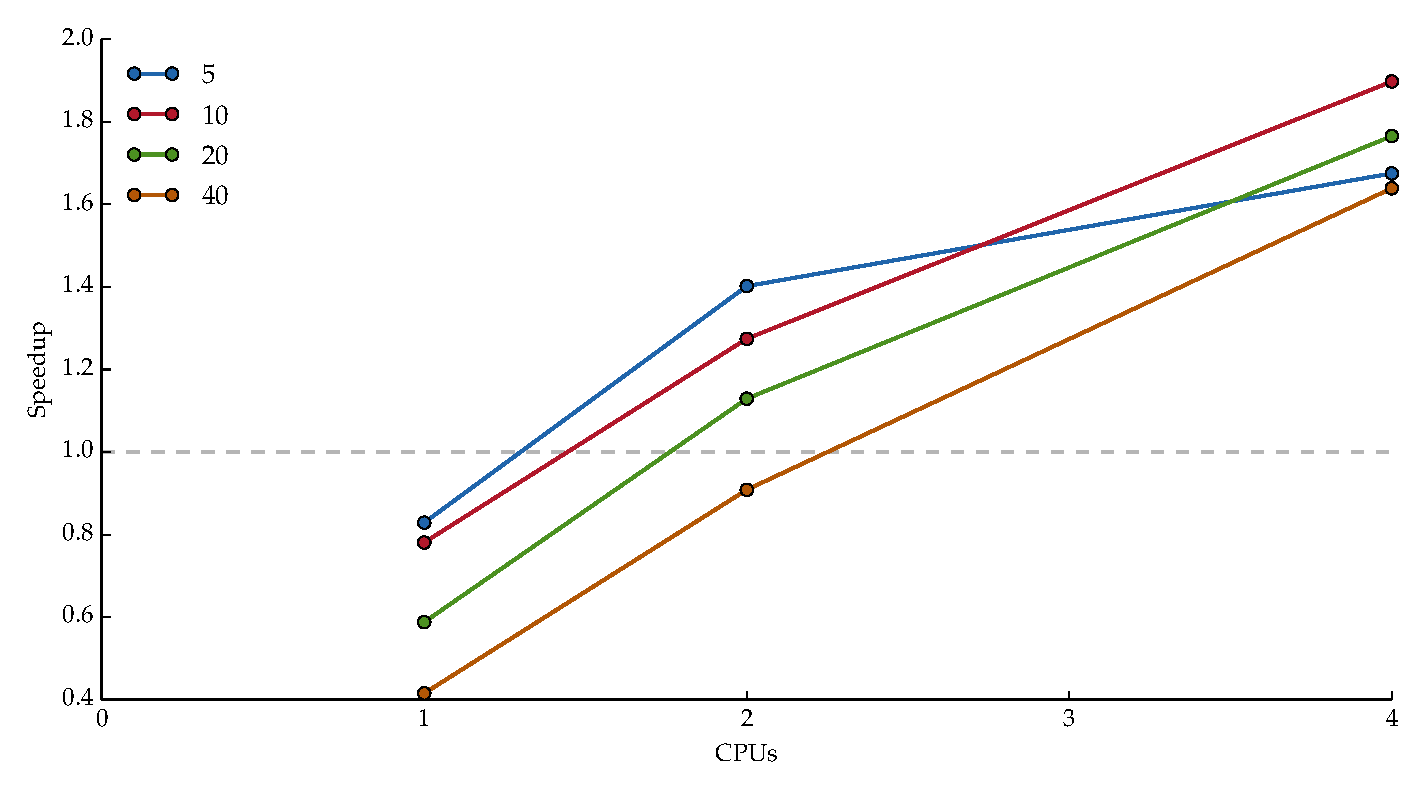
\includegraphics[width=\linewidth]{figs/10_appendices/speedup_cpus.pdf}
      \caption{
      Speedup of parallelised computation versus number of \textsc{cpu}s for
      different numbers of velocity classes $N_\Delta = \{ 5, 10, 20, 40 \}$,
      relative to the serial algorithm. Each data point is `best of two' to
      avoid times where the \textsc{cpu}s might otherwise be used by the
      operating system.
      }
      \label{fig:parallel_delta} 
    \end{figure}

    In figure \ref{fig:parallel_delta} we present measured speedup of
    parallelised computation with increasing number of \textsc{cpu} for example
    simulations using $5$, $10$, $20$ and $40$ velocity classes, relative to the
    serial code.

    We see that, for all numbers of velocity classes tested, using the parallel
    code but only allowing use of a single \textsc{cpu} incurs a slowdown due
    to the overhead of passing objects into the parallelised functions.

    In general the speedup decreases with the number of velocity classes, which
    indicates that there is significant overhead in parallelisation. With $2$
    \textsc{cpu}s we have speedup up to the case of $20$ velocity classes. With
    4 \textsc{cpu}s, the parallel algorithm results in significant speedup,
    above $60\%$ in each case. The speedup for $5$ velocity classes with $4$
    \textsc{cpu}s or more is obviously limited.

    The Lindblad solver routine in the velocity class loop represents the most
    computationally-intensive part of the whole algorithm, so it is certainly
    useful to be able to make use of multiple core computers to perform these
    calculations. For the work described in this thesis we made use of an Intel
    Core i7 with up to 4 \textsc{cpu} cores, and for the most intensive
    calculations we used Durham University's \textit{Hamilton} \textsc{hpc}
    Cluster with up to 12 \textsc{cpu} cores for each simulation.

    Another process which could be computed in parallel is the iteration over
    timesteps $t_k$ (algorithm \ref{alg:mb}, line 7), which performs the
    weighted average over density matrix coherences to determine the
    polarisation of the medium at that time, and advances the field via the
    \textsc{ab} step. However, for the number of timesteps used in calculations
    we saw negligible speedup due to the high overhead required for this loop in
    passing arrays containing the polarisations and fields. In fact, for systems
    where less than $N_k = 1000$ timesteps are required for the necessary
    accuracy, this overhead caused the parallel implementation to be slower
    than the serial. It was therefore not used.

    For fields with many modes, loops over these modes could be parallelised for
    computing polarisation. In this work we have only needed to consider systems
    of one or few modes, so it was not appropriate to implement parallelisation
    here.
